%!TEX root =../LibroTipoETSI.tex
\chapter{Introducción}\label{chp-01}


\lettrine[lraise=-0.1, lines=2, loversize=0.2]{E}{n} las prácticas de laboratorio realizadas
por parte de alumnos durante la docencia de los cursos de Robótica del Departamento de Ingeniería
de Sistemas y Automática de la Escuela Técnica Superior de Ingeniería de Sevilla, los alumnos
deben programar el movimiento de un brazo robótico presente en dicho laboratorio. El objetivo
es que una pieza sea trasladada por el robot desde un punto de la mesa de trabajo hacia una
segunda posición. El proceso se realiza colocando manualmente la pieza, con los problemas que
ello conlleva. Por un lado, la precisión es cuestionable, ya que el propio alumno no tiene una
referencia sobre la cual poder repetir el proceso de forma eficaz y el error introducido al sistema
es alto. Por otro lado, al invadir el espacio de trabajo del brazo robótico continuamente se
producen riesgos innecesarios impropios de las normas de seguridad en la industria.

Este trabajo es la continuación de Tapia\cite{tapia} e Hinojosa\cite{rea}, que sentaron las bases del proyecto.
En esta ocasión, el enfoque es en la implementación sobre los equipos del laboratorio. Por ello,
el sistema creado debe quedar compacto en una caja donde se realicen las conexiones electrónicas y todos
los dispositivos. Además el sistema debe tener componentes fácilmente sustituibles para facilitar
las reparaciones.

El sistema cuenta con las siguientes características:
\begin{itemize}
	\item Posicionamiento de piezas en medidas de ejes X e Y que el usuario requiera para 
	interactuar con el robot.
	\item Conexión entre Arduino y RobotStudio mediante protocolo TCP/IP para comunicaciones.
	\item Funcionamiento sin Arduino mediante señales digitales del robot.
	\item Funcionamiento sin conexión directa entre RobotStudio y Arduino.
\end{itemize}

\section{Modos de funcionamiento}\label{sec-00}

Todas las características especificadas previamente no pueden cumplirse al mismo tiempo ya que 
existirían conflictos entre las mismas, por lo que el sistema debe tener modos de funcionamiento 
específicos y diferenciados en los que se activen o desactiven dichas características. 

La primera consideración es determinar el dispositivo que gobierna el sistema o \textit{máster}.
Por ello, se puede diferenciar cuando el máster es la controladora del robot (o RobotStudio durante
una simulación) o el sistema caja (Arduino o la propia electrónica interna). Respectivamente serán
los modos remoto y local.

Por otro lado, como el microcontrolador presente en el Arduino puede estar funcionando o no, se
deben añadir las dos posibilidades. Se tiene el modo con microcontrolador y sin microcontrolador.

En total, se cuenta con cuatro modos de funcionamiento que se describen a continuación.

\subsection{Modo local con microcontrolador}\label{subsec-01}

Las órdenes del sistema están proporcionadas por los periféricos de entrada como pueden ser los botones
o interruptores bipolares presentes en la caja, mientras que el microcontrolador es el encargado de 
gestionar el posicionamiento y mover el motor cuando le sea indicado.

En caso de que esté disponible la conexión con la controladora del robot, el Arduino comunica 
mediante conexión TCP/IP la posición de la pieza en los ejes X e Y además del estado
del sensor fotoeléctrico y del sistema.

\subsection{Modo remoto con microcontrolador}\label{subsec-02}

El gobierno del sistema pasa a ser parte de la controladora del robot, convirtiendo al microcontrolador
en esclavo. El microcontrolador sigue encargándose del posicionamiento y movimiento del motor, pero las
órdenes pasan a ser recibidas mediante conexión TCP/IP.

Como en el caso anterior, se envía la posición, estado del sistema y del sensor fotoeléctrico mediante
conexión TCP/IP a la controladora.

\subsection{Modo local sin microcontrolador}\label{subsec-03}

Al no tener el microcontrolador operativo, el posicionamiento deja de funcionar y las funciones del
sistema pasan a ser más básicas. El movimiento del motor queda a cargo de la electrónica interna del
sistema. Para interactuar con el motor y moverlo se realizará mediante los pulsadores de avance y 
retroceso.

El robot queda no comunicado y solo recibe las señales digitales.

\subsection{Modo remoto sin microcontrolador}\label{subsec-04}

Este modo comparte la mayoría de características con el anterior y, físicamente es idéntico. La 
única diferencia es en el modo de uso, ya que que el control del movimiento de la cinta se realiza
con las señales digitales de avance y retroceso que permiten el movimiento.

\section{Distribución de los controles}

Para una interacción con el sistema se crea una interfaz hombre-máquina que permite cambiar entre los
distintos modos de funcionamiento, visualizar información, controlar el sistema en el modo local y realizar
paradas de emergencia en caso de ser necesario. Para ello, se prototipa la interfaz mostrada en la figura 
\ref{fig:interfazhmi}, que posteriormente se aplicará en el diseño de la caja.

En este diseño se observa un LCD que será el encargado de mostrar la información relevante como la posición o
el modo en el que se encuentra el sistema. Por otra parte, hay dos botones y una flecha de selección
que permiten avanzar por los distintos menús y seleccionar las opciones durante el modo local. Además, las flechas
serán las responsables del movimiento en el modo sin microcontrolador local. También se dispone de dos interruptores
de dos posiciones que permiten seleccionar los modos "local/remoto" y "con microcontrolador/sin microcontrolador".
Por último, una seta de emergencia es imprescindible para realizar una parada de emergencia en caso necesario. La 
seta está situada en un lugar de fácil acceso y que no interfiera en el uso normal del sistema.

\begin{figure}[htbp]
	\centering
	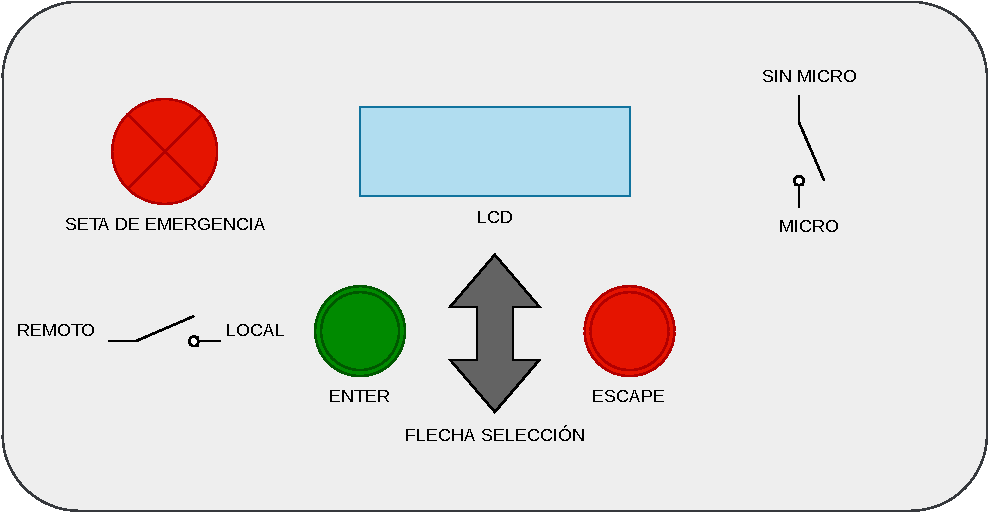
\includegraphics[width=\textwidth]{01-introduccion/HMI.pdf}
	\caption{Interfaz hombre-máquina. Distribución en la tapa.}
	\label{fig:interfazhmi}
	\end{figure}

Además, se debe crear una serie de conexiones que permitan la interacción robot-cinta para el modo remoto sin microcontrolador.
Esto se debe realizar mediante un conector que permita acceder a dichos pines de forma sencilla y queden expuestos.
Para ello, se introducirá un conector similar a la figura \ref{fig:digitales}. Los pines que debe contener son:
\begin{itemize}
	\item Retroceso.
 	\item Avance.
	\item Local.
	\item Micro.
	\item Emergencia.
  	\item Fotoeléctrico.	
\end{itemize}

\begin{figure}[htbp]
	\centering
	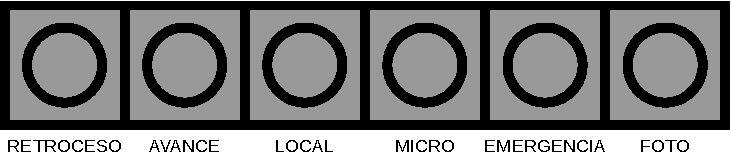
\includegraphics[scale=0.75]{01-introduccion/DIGITALES.pdf}
	\caption{Distribución de conexiones digitales}
	\label{fig:digitales}
	\end{figure}